\chapter{Gazelle View}
\label{chap:gazelleView}
 Gazelle View is the software developed in this project. 
 \begin{figure}[H]
 	\centering
 	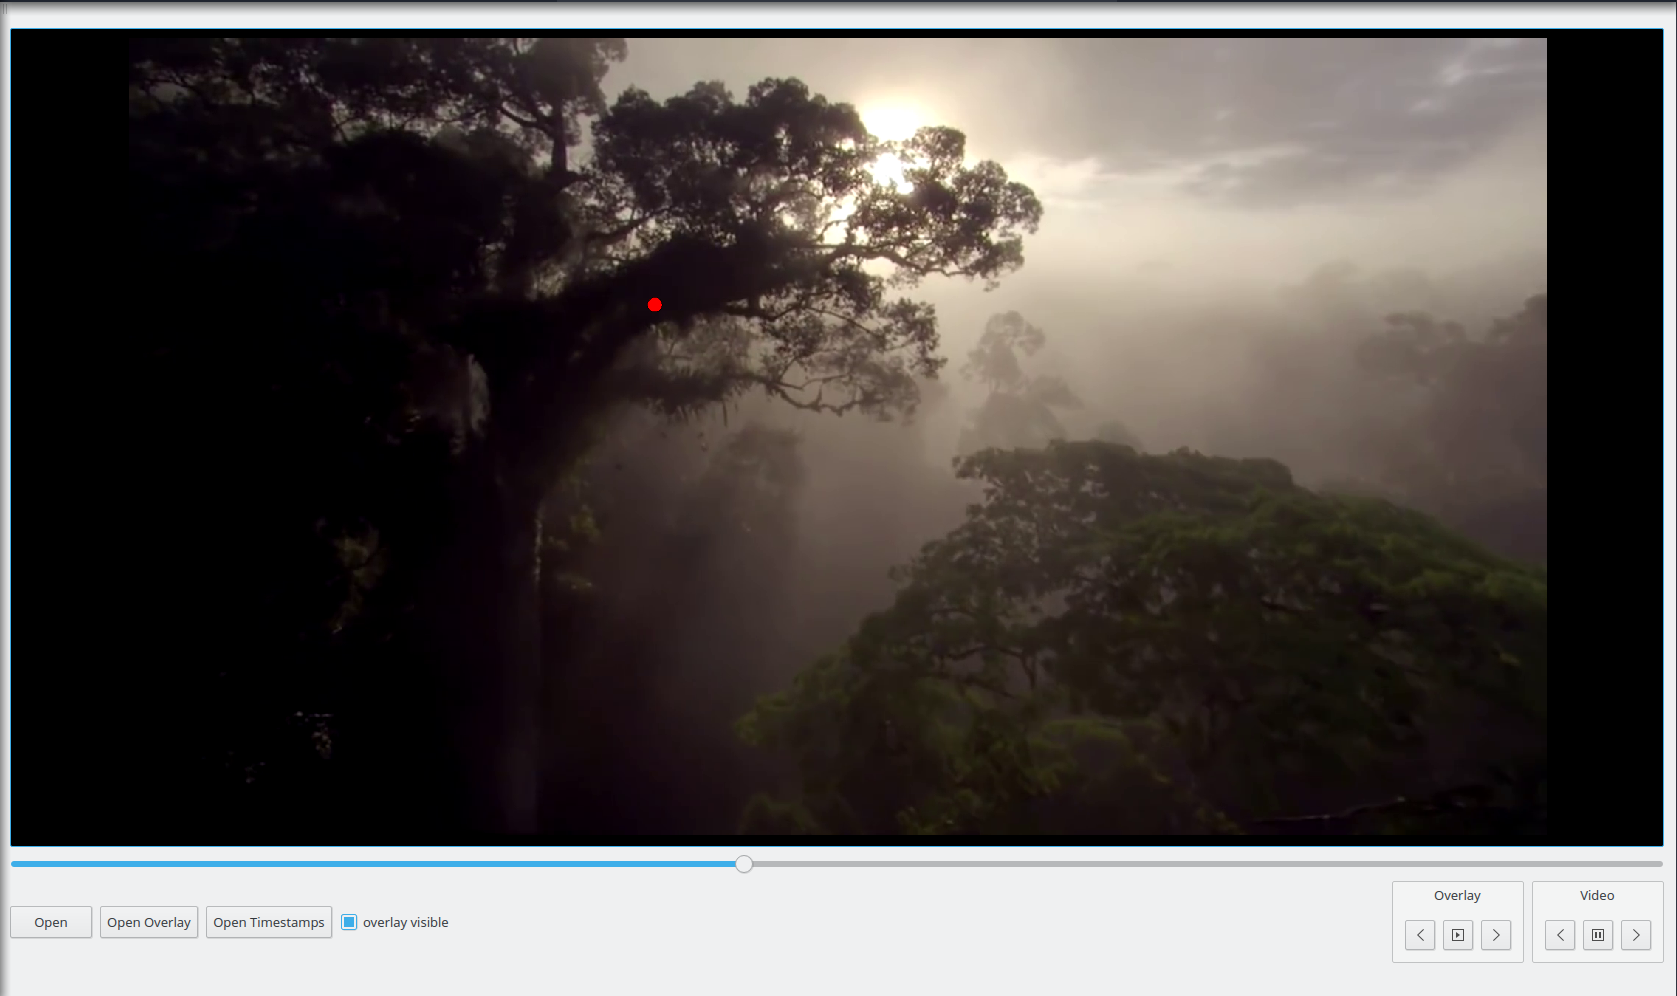
\includegraphics[scale=0.25]{images/gui_gazelle_view.png}
 	\caption{GUI of Gazelle View with the Breeze icon theme}
 	\label{fig:guiGazelleView}
 \end{figure}
\section{Use cases}
\label{sec:useCases}
The use cases for Gazelle View are presented in \ref{fig:useCases} and are deducted from the requirements.
\begin{itemize}
	\item The user can open a video, overlays and timestamps
	\item The user can play the video
	\item The user can pause the video
	\item The user can go to the next or previous frame
	\item The user can play overlays
	\item The user can pause overlays
	\item The user can go to the next or previous overlay
\end{itemize}
\section{Class Diagram}
Gazelle View is build with four classes as seen in \ref{fig:classDIagram} The GUI is handled by the class MainWindow. User input is forwarded to the class VideoHandler. VideoHandler is in control of which overlay and frame are displayed or decoded and it also manages the buffer. Because decoding is an expensive operation, so VideoHandler orders frames to be decoded from DecodeWorker. DecodeWorker has as sole instance access to the videostream and has to provide metadata such as framerate and how total count of frames in the stream. DecodeWorker runs in it's own thread so it doesn't block the other classes. The class Overlays is responsible to parse overlays and timestamps and find the corresponding frame or overlay for a timestamp.
\subsection{MainWindow}
\label{sec:mainWindow}
MainWindow handles the GUI, user input and displays the image with the overlay. It extends from QMainWindow and allows using the signal/slot framework from Qt. 
MainWindow sets up the icons of the play/pause, back and forwards buttons for overlay and video so that they use the icon theme of the current desktop environment. Fallback icons are provided for system that don't have themes or themes that don't have the necessary icons. An example of the GUI with the Breeze icon theme from KDE can be seen in \ref{fig:guiGazelleView}.

The communication with the class VideoHandler is done over the signal/slot framework from qt. The slot "displayImage" gets called when VideoHandler want's to display a new image. This image is shown on a QGraphicsScene with black background.
\subsection{VideoHandler}
\label{sec:videoHanlder}
VideoHandler handles a few things.
\begin{itemize}
	\item Order new frames to be decoded
	\item Send a frame to be displayed
	\item Handle the framebuffer
	\item Keep overlays and Frames in sync
	\item Send overlays to be displayed
\end{itemize}
VideoHandler extends QObject to communicate with the other classes over the signal/slot framework.

VideoHandler relies on DecodeWorker to decode the frames in a separate thread and on Overlays for getting the information which overlay needs to be displayed on which frame.
\subsubsection{Framebuffer}
\label{sec:framebuffer}
As decided in \ref{sec:frameBuffer} this is done with a QHash with the framenumber as key and a pointer to the Image as value. The buffer is trailing so it stores the last 50-100 frames. This is because the stream can only be decoded forward and jumping to a previous frame is expensive. To keep the size of the framebuffer reasonable a method iterates over the QHash when it get's to large and deletes all frames that are more than 50 frames behind.
\section{Overlay}
\label{sec:overlayClass}
The class Overlays is responsible for the following things.
\begin{itemize}
	\item parse file with information about overlays
	\item parse file of timestamps for the frames
	\item store overlays and timestamps
	\item return the overlay before or after a timestamp
	\item return the frame before a timestamp
	\item return the timestamp for a certain frame
\end{itemize}
The unit of the timestamps don't matter as long as they are the same for overlays and frames. 
As discussed in \ref{sec:overlays} a QMap stores the information for the overlays. The next or previous overlay is accessible for a timestamp. Additionally the corresponding timestamp for the overlay is also returned.
\subsection{Timestamps for Frames}
\label{sec:timestampsForFrames}
It is required to provide access for both the timestamp for a certain frame and the frame for a certain timestamp. In \ref{sec:timestamps} successive approximation was proposed to solve this issue. The implementation is as follows:

\begin{lstlisting}
for (int i = 2; i <= size; i *= 2) {
	if ((frameCount > (currentFrame + size / i)) &&
		(_sceneFrames.at(currentFrame + size / i) < timestamp)) {
		currentFrame += size / i;
	}
}
\end{lstlisting}
\begin{itemize}
	\item \texttt{\_sceneFrames} is the QVector that stores timestamps
	\item \texttt{frameCount} is the size of \texttt{\_sceneFrames}
	\item \texttt{size} is the next higher power of two after \texttt{frameCount}
	\item \texttt{currentFrame} holds the result at the end of the algorithm
	\item \texttt{currentFrame + size / i} is the frameindex that is tested
\end{itemize}
The result converges to the frameindex that has the timestamp below the timestamp that is supplied. It does so by comparing the supplied timestamp with the timestamp at index $\displaystyle\frac{\mbox{\texttt{size}}}{\mbox{2}}$ of \texttt{\_sceneFrames} first and followed by either $\displaystyle\frac{\mbox{\texttt{size}}}{\mbox{4}}$ or $\displaystyle\frac{\mbox{3 x \texttt{size}}}{\mbox{4}}$ depending on the outcome of the comparison. This goes on until the increment is one.

%The index doubles every iteration and the target timestamp is compared with the %timestamp at the frameindex of the current iteration. Access to  to non-existent %entries are prevented by comparing the frameindex to the size of %\texttt{\_sceneFrames}. The resulting frameindex is set to the tested frameindex %when the timestamp at said index is smaller than the reference timestamp. Otherwise %\texttt{currentFrame} stays the same. 

\section{Glossay}
\label{sec:instructions_glossay}

A glossary\index{glossary} can also be created in \LaTeX{} with the \texttt{makeindex} program and the \texttt{glossaries} package. The following list shows the procedure to generate a glossary:

\begin{itemize}
	\item Integration of the package \texttt{glossaries}.
	\item If necessary, a personal database may be created including glossary entries. This template works with such a database, which is stored in the \texttt{database}folder. Entries from the database are only written in the directory if the word in the text is actually stated.
	\item With the \texttt{\textbackslash makeglossaries} command a new compilation is initialized.
	\item New entries can be created with the command \\ \texttt{\textbackslash newglossaryentry\{<SHORTCUT>\}\{name=\{<NAME>\},description=\{<DESCRIPTION>\}\}}.
	\item In the text continuously referencing words with the command \texttt{\textbackslash gls\{<SHORTCUT>\}}.
	\item Similar to the compilation of the index, the directory is only embedded into the document  during the second passage.
\end{itemize}

In order to work accurately, the glossary must be compiled with \texttt{makeindex} after post-editing the document. For this the following code in the command line is to be executed:

\begin{center}
	\texttt{makeindex -s template.ist -t template.glg -o template.gls template.glo}
\end{center}

With most \LaTeX editors, this can be stated as a post-processing step. The following explanation is for the TeXnicCenter program. Under the menu "Build" > "Define Output Profile..." (short: alt + F7) in the "Postprocessor" register, the window shown in Figure \ref{fig:postprocessing} can be found. Then it is necessary to insert a new entry, when an application as well as an argument must be specified. The application can be found in the MiKTeX installation (\texttt{..\textbackslash MiKTeX X.X\textbackslash miktex\textbackslash bin\textbackslash makeindex.exe}). As an argument, the following line must be entered:

\begin{center}
	\texttt{-s \string"\%tm.ist\string" -t \string"\%tm.glg\string" -o \string"\%tm.gls\string" \string"\%tm.glo\string" }
\end{center}

\begin{figure}[H]
	\centering
		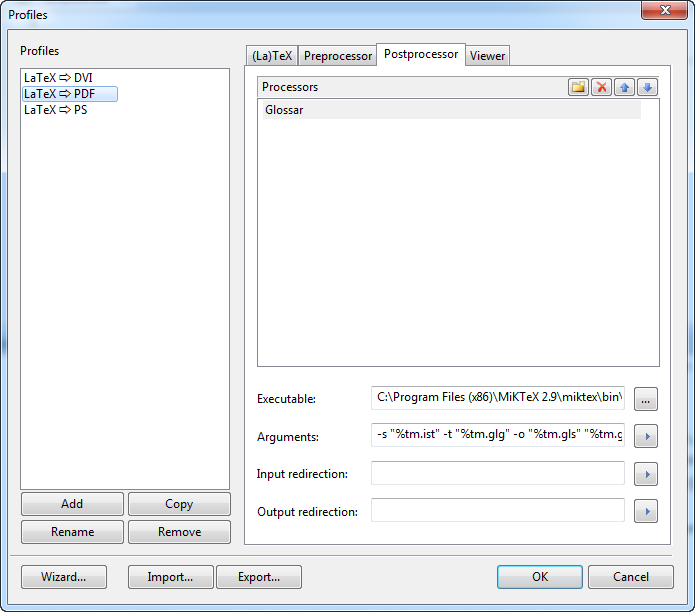
\includegraphics[scale=0.6]{images/profiles_glossar.png}
	\caption{Post-processing}
	\label{fig:postprocessing}
\end{figure}


\section{Bibliography}
\label{sec:instructions_bibliography}

To compile a bibliography\index{bibliography} one must resort to \gls{BibTeX}. The folder \texttt{database} includes a \texttt{.bib} file with various database entries. How the entries are to be compiled, can be taken from various sources of the Internet or books. The entries in the database will only be written to the directory of the document when the source is actually cited in the text.

Under the following addresses further explanations are found in order to compile the database and its use:

\begin{itemize}
	\item \url{http://en.wikipedia.org/wiki/BibTeX}
	\item \url{http://www.bibtex.org/}
\end{itemize}


